\section{Hardware Analyse und Festlegung}

\subsection {Hardware Analyse}

Im Folgenden wird die Hardware und Bauteil Analyse näher beschrieben.
 Diese folgt zu den Designentscheidungen und ist ein wichtiger Bestandteil, um bestimmte Anforderungen zu erfüllen.
 
 Wie im vorherigen Teil bereits erläutert gibt es nahezu unendlich viele Szenarien, in denen ein Rescue Roboter eingesetzt werden kann. 
Das Projekt befasst sich mit dem Szenario eines Brands, in dem eine Person gerettet werden muss. Dabei muss der Roboter in der Lage sein, Hindernisse wegzuräumen und zu passieren. 
Zudem muss dieser an Land fahren können und auch Wasser überqueren.
Des Weiteren soll der Roboter in der Lage mit einer Person zu kommunizieren. 
Hierfür gibt es eine Anforderungsliste und ein bestimmtes Use-Case.
Daraus geht hervor das unterschiedlichste Aufgaben zu bewältigen sind.
Diese müssen nachweisbar zu belegen sein. 

 Bei der Konstruktion eines Konzept Roboters für den realen Gebrauch, gibt es verschiedene Bereiche. 
Sowohl Software-technische Bereiche als auch Hardware-technische Bereiche. Die folgende Analyse befasst sich mit den Hardware-Anforderungen. 
Zu Beginn der Hardware und Mechanik Analyse wurde eine Tabelle erstellt. 
Diese listet verschiedene Bauteile auf und zeigt die Vor- und Nachteile. 
Zudem gibt es eine Zusammenfassung mit der Nutzbarkeit für das oben beschriebene Use Case. 
Nach der Analyse folgte eine darauf basierende Entscheidung wie das Design und der Roboter konzipiert sind. 


\begin{figure} [ht]
\begin{center}
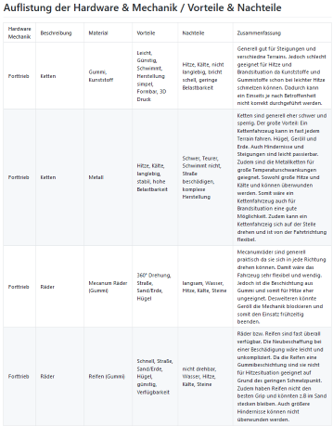
\includegraphics [width = 0.4\textwidth] {HW1.png}
\caption {Auflistung der Hardware und Mechanik /Vor- und Nachteile (1)}
\end {center}
\end {figure}

\begin{figure} [ht]
\begin{center}
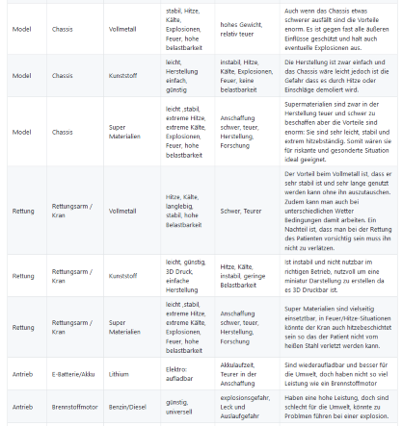
\includegraphics [width = 0.4\textwidth] {HW2.png}
\caption {Auflistung der Hardware und Mechanik /Vor- und Nachteile (2)}
\end {center}
\end {figure}

\subsection {Forttrieb}
Als erster Teilbereich wurde der Forttrieb an Land untersucht. 
Hier wurden Ketten, normale Reifen und Mecanum-Räder untersucht. 
Auch wenn die Ketten schwer sind, haben Sie doch einen großen Vorteil gegenüber den anderen beiden Typen. 
Sie sind robust und hitzebeständig. In dem Szenario gibt es ein Feuer und brennende Hindernisse.
Dabei gibt es eine hohe Temperaturentwicklung. 
Für den Fall, dass gummierte Reifen eingesetzt werden, könnten diese schmelzen.
Wenn dies eintritt verlieren Reifen ihre Funktionalität und ein korrekter Einsatz muss gegebenenfalls frühzeitig beendet werden. 

Somit ist die Auswahl auf robuste Ketten gefallen.
Ein weiterer Vorteil ist die Steigung und Passierbarkeit von Hindernissen. 
Durch einen Kettenantrieb ist es möglich über Geröll und verschiedene Bodentypen zu fahren, ohne sich festzufahren.
Wenn der Roboter auch durch einen See fahren soll, hat der Roboter mit Kettenantrieb, an dem Ufer mehr Grip und kann besser hinein- und herausfahren. 

\subsection {Chassis}
An zweiter Stelle wurde das  Chassis und dazu gehörige Material genauer betrachtet. 
Das Gehäuse und die Beschaffenheit hängen stark mit den Anforderungen zusammen. 
Zwar ist ein Roboter aus 3D gedrucktem Material leichter und schnell gefertigt, doch so gibt es auch hier einen wichtigen Nachteil. 
Der Schmelzpunkt von 3D Drucken und üblichen Kunststoffen ist recht gering.
Im Falle eines Brandes könnte das Gehäuse schmelzen und das Fahrzeug in sich kollabieren.

Metall wäre besser geeignet ist aber nicht auch nicht optimal. 
Das hohe Gewicht wirkt sich auf den gesamten Roboter aus. 
Da der Rescue Roboter schwimmen soll, ist das Gewicht relativ gering zu halten, wenn möglich.
Das Gehäuse könnte aus einem Supermaterial gefertigt werden, wie in der Raketenforschung. 
Dort gibt es ein leichtes Material welches als Hitzeschild benutzt wird aber dennoch leicht ist. 
Wie zum Beispiel Kohlefaser-Verbundstoff mit einer Keramikbeschichtung. 
Diese Materialien sind zwar teuer in der Herstellung und Produktion aber für einen speziell konstruierten Rescue Roboter von großem Vorteil. 

\subsection {Rettungsvorgang}
Als nächstes wurde der Rettungsvorgang analysiert. 
Hierfür eignet sich ein multifunktionaler Greifarm am besten.
In dem Szenario sollen Hindernisse weggeräumt werden. 
Zudem sollen Personen gerettet und versorgt werden. 
Mit einem ferngesteuerten Roboter-Greifarm der sich in mehrere Richtungen drehen und ausfahren kann, könnte dies realisiert werden. 
Das Material sollte auch hier wieder ähnlich speziell gewählt sein wie bei dem Chassis wegen der hohen Hitze. 
Um den Greifarm in mehrere Richtungen zu drehen und auszufahren werden drei unabhängige Motoren verwendet, um die geeignete Leistung aufzubringen.
Für den Rettungsvorgang ist eine nach oben öffnende Doppeltür-Klappe vorgesehen. 
Diese kann sich öffnen, um zum Beispiel Verbandskästen mithilfe des Krans herauszugeben oder eine zu rettende Person, dort im Innenraum aus der Gefahrensituation zu befördern.

\subsection{Energieversorgung und Motoren}
Die Energie Versorgung soll über E-Akkus erfolgen. 
Die Motoren agieren ebenfalls über elektrische Leistung. 
Die benutzten Elektro-Motoren und Akkus sind speziell beschichtet, um der Hitze Stand zu halten. 

Es werden kein Benzin/Diesel oder Öl-Tanks und Motoren verwendet da diese das Risiko haben bei hoher Hitze zu explodieren. 
Zudem dürften diese kein Leck haben. 
Durch austretendes Benzin könnten Brandpfützen entstehen. 
Des Weiteren könnte das Wasser verunreinigt werden.

\subsection{Forttrieb im Wasser}
Um den Forttrieb im Wasser zu gewährleisten werden mehrere Aspekte berücksichtigt. 
Der Rescue Roboter verfügt über eine hinten angebrachte Schiffschraube, auf einer höhenverstellbaren Schiene.
Mit Hilfe dieser, kann die Schiffsschraube auf die gewünschte Höhe gebracht werden, so wie auf- und abgelassen werden, je nach Umgebung.
Damit kann der Robot sich im Wasser vorwärtsbewegen. 

Um einen generellen Auftrieb zu geben, verfügt der Roboter über einen großen Luft-Hohlraum. Dieser fungiert ähnlich wie bei einem Schiff und gibt dem Roboter die Möglichkeit besser zu schwimmen. Für den weiteren Auftrieb nach oben sorgt eine leistungsstarke Pumpe die mittels Düsen, Wasser einsaugt und nach unten ausströmt. Des Weiteren befindet sich unten am Roboter ein Feuchtigkeitssensor, um zwischen Land- und Wasser zu wechseln. 

\subsection{Raumaufteilung}
Der Roboter besteht aus drei Haupträumen. 
Der oberste dient zur Personenrettung und verfügt über eine Türklappe.
In diesem Raum ist die Person vor äußeren Einflüssen geschützt. Zudem befindet sich dort ein Erste-Hilfe-Kasten. 
Der mittlere Raum ist der Technik-Raum bzw. Motoren-Raum, welcher über eine hintere Tür für Wartungsarbeiten zugänglich ist. 
Der unterste Raum ist als Hohlraum für den Wasserauftrieb konzipiert.

\subsection {Technische Komponenten}
Da der Rescue Roboter noch weitere Anforderungen besitzt, werden diese im Weiteren erläutert. 
Der Roboter muss mit dem Umweltsystem interagieren und kommunizieren können.
Dafür gibt es mehrere Möglichkeiten dies zu realisieren. 
Verschiedene Technikkomponenten kommen zum Einsatz. 

\subsection {Orientierung}
Um mit der Einsatzleitung zu kommunizieren und generelle Signale senden und empfangen zu können ist eine Antenne angebracht. 
Zur generellen Orientierung gibt es ein GPS mit integriertem Kompass.
Für die lokale Orientierung von Hindernissen und Wegen sind acht Abstandssensoren am Roboter befestigt. 
Diese blicken in verschiedene Richtungen und scannen die Umgebung. 
Die Daten werden über die Software analysiert und berücksichtigt.

\subsection {Display und LED}
Für eine verbesserte Sicht bei eingeschränkten oder dunklen Begebenheiten sind vorne drei LED-Scheinwerfer angebracht. Damit der Roboter und der Operator mit der zu rettenden Person kommunizieren können ist vorne ein großes Display angebracht. Über dieses lassen sich Instruktionen und Video Chats anzeigen.

\subsection {Multimediaglobe und Kameras} 
Damit der Operator noch besser mit der Person kommunizieren kann, ist ein Multimedia-Globe vorne im Greifarm eingebaut.
In diesem Globe befindet sich ein Mikrofon, ein Lautsprecher und eine Kamera. 
So kann der Greifarm nah an die Person heranfahren und mit ihr audio-visuell den Kontakt aufnehmen.
 
Vorne am Roboter ist ein spezielles Kamera Array angebracht. Dieses verfügt über verschiedene Kameras und Techniken.  
So gibt es eine digitale Kamera für die generelle Bildübertragung. Zudem gibt es eine Thermalkamera und Infrarotkamera, welche die Temperaturgegebenheiten anzeigen können. 
Des Weiteren gibt es eine Nachtsichtkamera, um auch in dunklen Bereichen ein visuelles Bild zu übertragen. 

Diese Techniken werden von verschiedenen Einsatzkräften bei Millitär und Feuerwehr eingesetzt. Dabei werden verschiedene Systeme benutzt um mögliche Szenarien abzudecken. Die Vielseitgkeit erlaubt es zwischen unterschiedlichen Sehbereichen zu wechseln, um das Ziel zu erreichen.

\subsection {Reale Umsetzung} 
Die Hardware und Bauteilanalyse wurden für Designentscheidungen berücksichtigt und umgesetzt.
Der Rescue Roboter verfügt über die in den Anforderungen beschriebenen Bestandteile.
Da es sich um ein Konzept Entwurf handelt ist die grobe Richtung eingeleitet. 
Bis hin zur finalen Realisierung muss der Entwurf iterativ verfeinert werden.
Der Rescue Roboter ist in der Planung ein Unikat und als Projekt zu verstehen.
Für das Konstruieren werden spezielle Materialien und Sensoriken benötigt.
Diese müssen teils extra gefertigt und bestellt werden. 
Da es sich um einen Roboter für Extremsituationen handelt in dem Menschen gerettet werden, ist die Planung enorm wichtig und muss mit mehreren Gremien und Sachverständigen geplant werden.
Die Anforderungen und Richtlinien sind dabei hoch und vielschichtig komplex.  




